\documentclass[addpoints, 12pt, answers]{exam}

\usepackage{epstopdf}
\usepackage{makecell}

\usepackage{mathtools}
\usepackage{wrapfig}
\usepackage{tabularx}
\usepackage{multirow}
\usepackage{tikz}
\usepackage{circuitikz}
\usepackage{float}

\usepackage{setspace}

\usepackage[margin=1in]{geometry}
\usepackage{amsmath,amsthm,amssymb,amsfonts}

\usepackage[ruled,boxed,algo2e]{algorithm2e}
\usepackage{algorithm}
\usepackage{pifont}
\usepackage{graphicx}
\usepackage{listings}
\usepackage{color}

\usepackage{array}

\usepackage{booktabs}

\usepackage{amsmath,amscd}
\usepackage{amssymb,array}
\usepackage{amsfonts,latexsym}
\usepackage{graphicx,subfig,wrapfig}
\usepackage{times}
\usepackage{psfrag,epsfig}
\usepackage{verbatim}
\usepackage{tabularx}
\usepackage{makecell}
\usepackage{graphics}
\usepackage{caption}

\usepackage{enumerate}
\usepackage{listings}

\usepackage{ulem}
\usepackage[pagebackref=true,breaklinks=true,letterpaper=true,colorlinks=false,bookmarks=false]{hyperref}

\usepackage{multicol}

\usepackage{lastpage}

\newcommand{\N}{\mathbb{N}}
\newcommand{\Z}{\mathbb{Z}}

\DeclareMathOperator*{\rank}{rank}
\DeclareMathOperator*{\trace}{trace}
\DeclareMathOperator*{\acos}{acos}
\DeclareMathOperator*{\argmax}{argmax}

\renewcommand{\mathbf}{\boldsymbol}
\newcommand{\mb}{\mathbf}
\newcommand{\matlab}[1]{\texttt{#1}}
\newcommand{\setname}[1]{\textsl{#1}}
\newcommand{\Ce}{\mathbb{C}}
\newcommand{\norm}[2]{\left\| #1 \right\|_{#2}}

\newcommand{\exercise}[2]{\item[] \textbf{Exercise #1 #2}}

\lstset{frame=none,
    language=c,
    aboveskip=3mm,
    belowskip=3mm,
    showstringspaces=false,
    columns=flexible,
    basicstyle={\small\ttfamily},
    numbers=left,
    numberstyle=\tiny\color{gray},
    keywordstyle=\color{blue},
    commentstyle=\color{dkgreen},
    stringstyle=\color{mauve},
    breaklines=true,
    breakatwhitespace=true,
    tabsize=8
}

\definecolor{dkgreen}{rgb}{0,0.6,0}
\definecolor{gray}{rgb}{0.5,0.5,0.5}
\definecolor{mauve}{rgb}{0.58,0,0.82}




\pagestyle{headandfoot}
\runningheadrule
\firstpageheader{Computer Architecture I}{Homework 8}{2023}
\runningheader{Email:}
{Homework, Page \thepage\ of \numpages}
{Computer Architecture I 2023}
\firstpagefooter{}{}{}
\runningfooter{}{}{}

\boxedpoints

\pointsinmargin



\setlength\answerlinelength{.95\linewidth}


\begin{document}
\begin{center}

{\centering \Large Homework 8\\\vspace{.75cm}}

\vspace{0.1cm}
\makebox[\textwidth]{Chinese Name:\enspace\hrulefill}\\[0.6cm]
\makebox[\textwidth]{Pinyin Name:\enspace\hrulefill}\\[0.6cm]
\makebox[\textwidth]{Student ID:\enspace\hrulefill}\\[0.6cm]
\makebox[\textwidth]{E-Mail ... @shanghaitech.edu.cn:\enspace\hrulefill}\\[0.5cm]

\end{center}


\begin{questions}

\question[10] \textbf{Put T (True) or F (False) for each of following statement. [10 points]}

\begin{enumerate}[(1)]
    \item ( \quad ) One of the main advantages of using virtual memory is that it allows the OS to use a single address space for all processes. 
    \item ( \quad  ) The translation lookside buffer (TLB) generally holds the most-recently-used page table entries that are used to translate memory page numbers to corresponding disk block numbers where pages are stored on disk.
    \item (\quad) The size of the virtual address space accessible to the program cannot be larger than the size of the physical address space.
    \item ( \quad  )  In practice, most of virtual memory systems in modern OS employ direct-mapped strategy to place memory pages for simplicity and low miss rate.
    \item (\quad) Page tables make it possible to store the pages of a program non-contiguously and add disk in the memory hierarchy
\end{enumerate}

\pagebreak
\question[20] \textbf{TLB Replacement [20 points]}

A processor has 16-bit addresses, 256 byte pages, 
and an 8-entry fully associative TLB with LRU replacement 
(the LRU field is 3 bits and encodes the order in which pages were accessed, 
0 being the most recent). 
At some time instant, 
the TLB for the current process is the initial state given in the~\autoref{tab:ini-tlb}. 
Assume that all current page table entries are in the initial TLB. 
Assume also that all pages can be read from and written to. 

Fill in the final state of the TLB in~\autoref{tab:fin-tlb} according to the access pattern in~\autoref{tab:access}. 
Free physical pages: 0x17, 0x18, 0x19.

\begin{table}[H]
	\centering
	\caption{Access Pattern for Memory}
	\label{tab:access}
	\begin{tabular}{|c|c|}
	\hline
	No. & Access Pattern \\ \hline
	1   & Write 0x2333   \\ \hline
	2   & Read 0x11F0    \\ \hline
	3   & Write 0x2023   \\ \hline
	4   & Write 0x1301   \\ \hline
	5   & Read 0x20FF    \\ \hline
	6   & Write 0x3415    \\ \hline
	\end{tabular}
\end{table}


\begin{table}[H]
	\begin{minipage}[t]{0.5\linewidth}
		\centering
			\caption{Initial TLB}
			\label{tab:ini-tlb}
			\begin{tabular}{|c|c|c|c|c|}
			\hline
			VPN  & PPN  & Valid & Dirty & LRU \\ \hline
			0x01 & 0x11 & 1     & 1     & 0   \\ \hline
			0x00 & 0x00 & 0     & 0     & 7   \\ \hline
			0x10 & 0x13 & 1     & 1     & 1   \\ \hline
			0x20 & 0x12 & 1     & 0     & 5   \\ \hline
			0x00 & 0x00 & 0     & 0     & 7   \\ \hline
			0x11 & 0x14 & 1     & 0     & 4   \\ \hline
			0xAC & 0x15 & 1     & 1     & 2   \\ \hline
			0xFF & 0x16 & 1     & 0     & 3   \\ \hline
			\end{tabular}
	\end{minipage}
	\begin{minipage}[t]{0.5\linewidth}
		\centering
		\caption{Final TLB}
		\label{tab:fin-tlb}
		\begin{tabular}{|c|c|c|c|c|}
		\hline
		VPN  & PPN  & Valid & Dirty & LRU \\ \hline
		 &  &      &      &    \\ \hline
		 &  &      &      &    \\ \hline
		 &  &      &      &    \\ \hline
		 &  &      &      &    \\ \hline
		 &  &      &      &    \\ \hline
		 &  &      &      &    \\ \hline
		 &  &      &      &    \\ \hline
		 &  &      &      &    \\ \hline
		\end{tabular}
	\end{minipage}
\end{table}



\pagebreak
\question[25] \textbf{Page Table Walk [25 points]}

Suppose there is a virtual memory system with 64KB page which has 2-level hierarchical page table. 
The {\em physical address} of the base of the level 1 page table (0x01000) is stored in the Page Table Base Register. 
The system uses {\em 20-bit} virtual address and {\em 20-bit} physical address. 
~\autoref{fig:pagetable} summarizes the page table structure in this system. 

\begin{figure}[h]
	\centering
	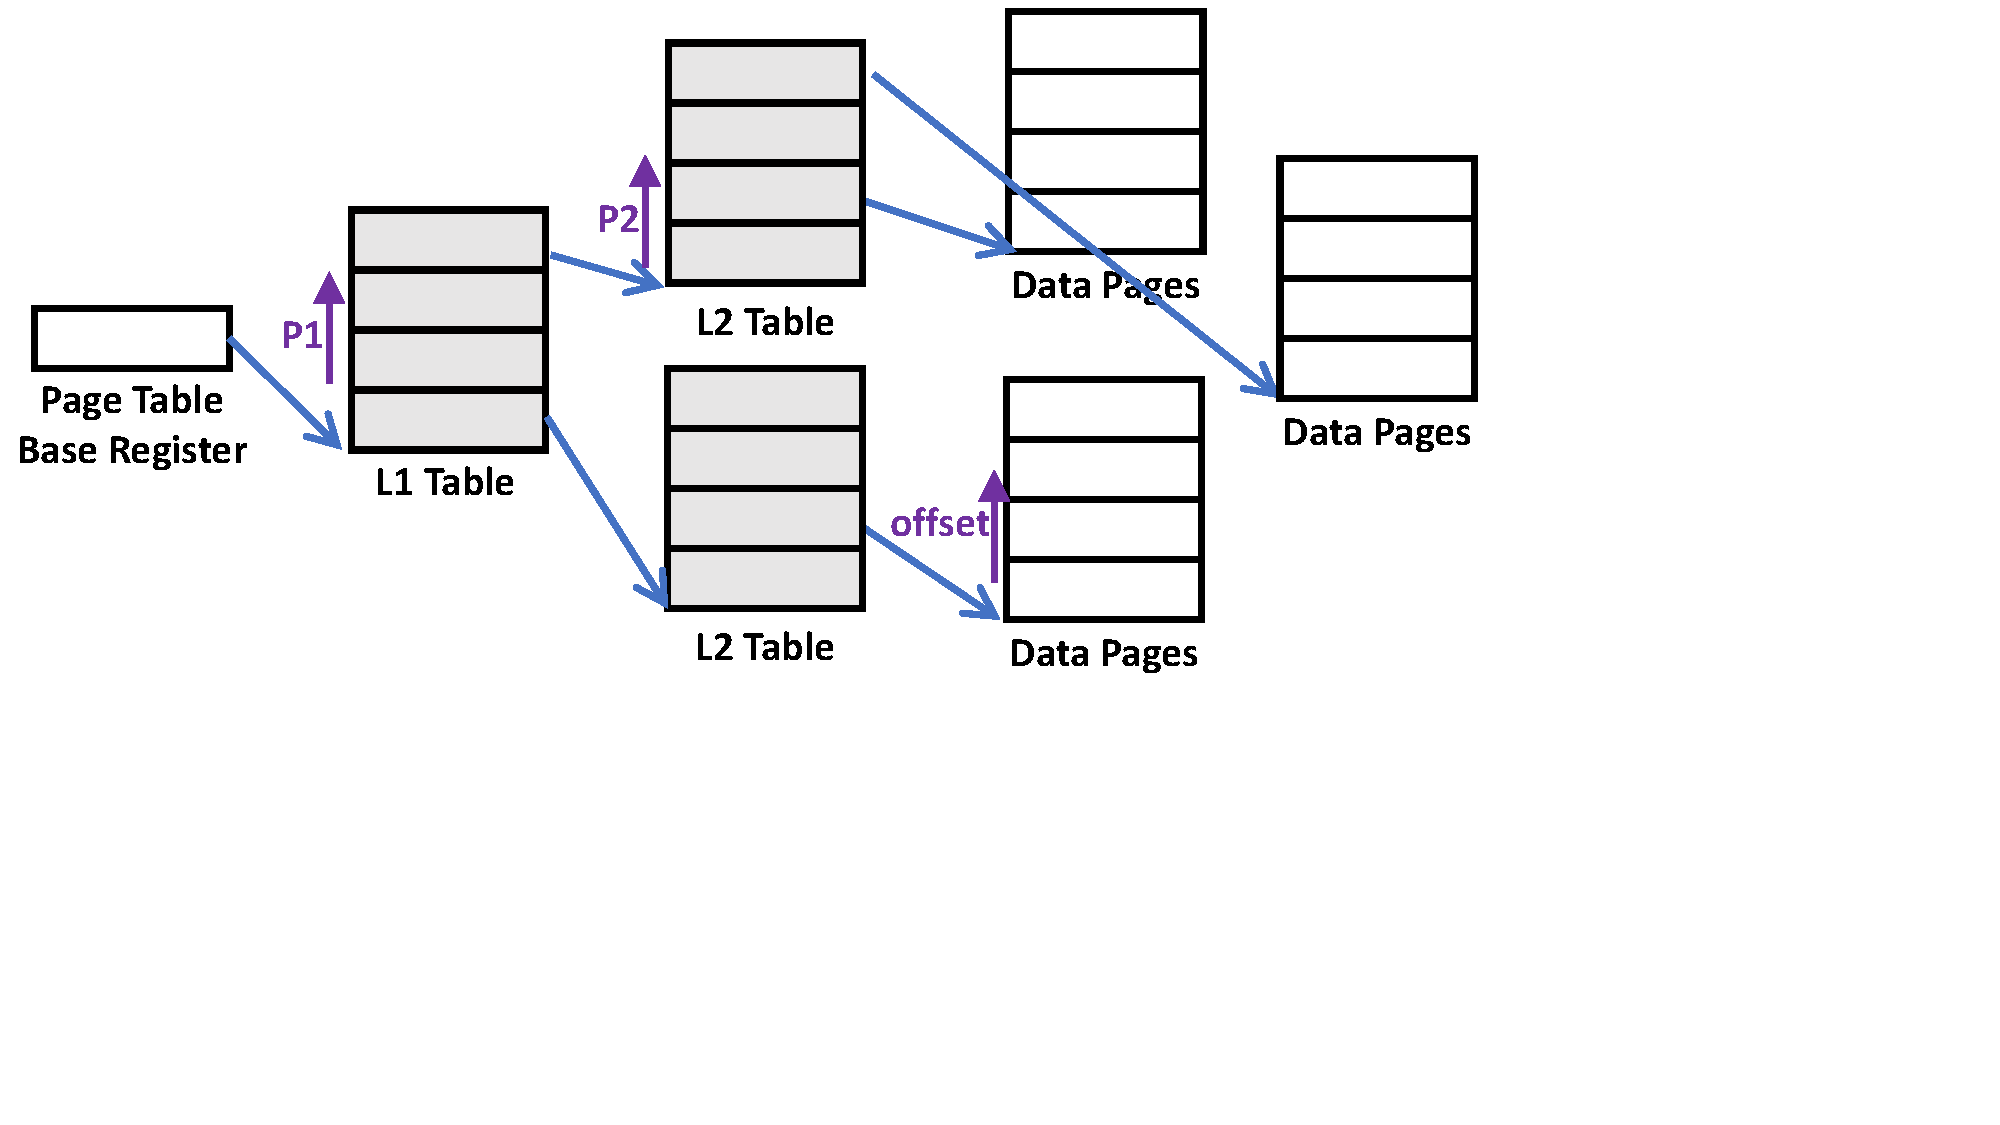
\includegraphics[width=0.8\columnwidth]{fig/pagetable.pdf}
	\caption{Two-level Hierarchical Page Table}\label{fig:pagetable}
\end{figure}


The size of both level 1 and level 2 page table entries is {\em 4 bytes} and the memory is byte-addressed. 
Assume that all pages and all page tables are loaded in the main memory. 
The breakdown of a virtual address is:

\begin{table}[h]
	\centering
	\begin{tabular}{lrlrlr}
	19 & 18 & 17 & 16 & 15 & 0 \\ \hline
	\multicolumn{2}{|c|}{L1 Index (p1)} & \multicolumn{2}{c|}{L2 Index (p2)} & \multicolumn{2}{c|}{\quad\quad\quad Page Offset \quad\quad\quad} \\ \hline
	\end{tabular}
\end{table}


Each entry of the level 1 page table contains the {\em physical address} of the base of each level 2 page tables, 
and each of the level 2 page table entries holds the PTE of the data page. 
As described in~\autoref{fig:pagetable}, L1 index and L2 index are used as an index 
to locate the corresponding {\em 4-byte entry} in Level 1 and Level 2 page tables.

A PTE in level 2 page tables can be broken into the following fields (Don’t worry about status
bits for the entire part).

\begin{table}[h]
	\centering
	\begin{tabular}{lrlrlr}
	31 & 20 & 19 & 16 & 15 & 0 \\ \hline
	\multicolumn{2}{|c|}{\quad\quad\quad\quad\quad\quad\quad\quad 0 \quad\quad\quad\quad\quad\quad\quad\quad} & \multicolumn{2}{c|}{Physical Page Number (PPN)} & \multicolumn{2}{c|}{Status Bits} \\ \hline
	\end{tabular}
\end{table}


\newpage

\begin{parts}

\part[10] \textbf{A [10 points]}

Assuming the initial TLB and memory states are in~\autoref{tab:a:ini-tlb} and~\autoref{tab:a:ini-mem}, respectively,  
what will be the final TLB states after accessing the virtual address given below? 
Please fill out the table with the final TLB states in~\autoref{tab:a:fin-tlb}. 
You only need to write VPN and PPN fields of the TLB. 
The TLB has 4 slots and is fully associative and 
if there are empty lines they are taken first for new entries. 
Also, translate the virtual address (VA) to the physical address (PA). 

\begin{table}[H]
	\begin{minipage}[t]{0.6\linewidth}
		\centering
		\caption{Initial TLB State}\label{tab:a:ini-tlb}
		\begin{tabular}{|c|c|}
		\hline
		\quad VPN \quad\quad & \quad PPN \quad\quad \\ \hline
		0x8 & 0x3 \\ \hline
		-- & -- \\ \hline
		-- & -- \\ \hline
		-- & -- \\ \hline
		\end{tabular}


		\quad\\ \quad\\

		\caption{Final TLB State}\label{tab:a:fin-tlb}
		\begin{tabular}{|c|c|}
		\hline
		\quad VPN \quad\quad& \quad PPN \quad\quad\\ \hline
		0x8 & 0x3 \\ \hline
		 &  \\ \hline
		 &  \\ \hline
		 &  \\ \hline
		\end{tabular}


		\quad\\ \quad\\


		VA: {\em 0xD180B} $\longrightarrow$ PA: \underline{\quad\quad\quad\quad\quad\quad\quad\quad}


		\end{minipage}
	\begin{minipage}[t]{0.4\linewidth}
		\centering
		\caption{Initial Memory State}\label{tab:a:ini-mem}
		\begin{tabular}{|c|c|}
		\hline
		Address (PA) & \quad Content \quad\quad \\ \hline
		0x0104C & 0x71A02 \\ \hline
		0x01048 & 0x30044 \\ \hline
		0x01044 & 0x20560 \\ \hline
		0x01040 & 0xA0FFF \\ \hline
		0x0103C & 0xCD031 \\ \hline
		0x01038 & 0xA6213 \\ \hline
		0x01034 & 0x91998 \\ \hline
		0x01030 & 0xDAB04 \\ \hline
		0x0102C & 0xFA000 \\ \hline
		0x01028 & 0x60020 \\ \hline
		0x01024 & 0x51040 \\ \hline
		0x01020 & 0x4AA40 \\ \hline
		0x0101C & 0x310EF \\ \hline
		0x01018 & 0xBEA46 \\ \hline
		0x01014 & 0x2061B \\ \hline
		0x01010 & 0x10040 \\ \hline
		0x0100C & 0x01020 \\ \hline
		0x01008 & 0x01048 \\ \hline
		0x01004 & 0x01010 \\ \hline
		0x01000 & 0x01038 \\ \hline
		\end{tabular}
		\end{minipage}
\end{table}



\part[15] \textbf{B [15 points]}

Li Hua wants to reduce the amount of physical memory required to store the page table,
so he decided to only put the level 1 page table in the physical memory 
and use the {\em virtual memory} to store level 2 page tables. 
Now, each entry of the level 1 page table 
contains the {\em virtual address} of the base of each level 2 page tables, 
and each of the level 2 page table entries contains the PTE of the data page. 
Other system specifications remain the same. 
(The size of both level 1 and level 2 page table entries is 4 bytes.) 

Assuming the initial TLB and memory states are in~\autoref{tab:b:ini-tlb} and~\autoref{tab:b:ini-mem}, respectively, 
what will be the final TLB states after accessing the virtual address given below? 
Please fill out the table with the final TLB states in~\autoref{tab:b:fin-tlb}.  
You only need to write VPN and PPN fields of the TLB. 
The TLB has 4 slots and it is fully associative and 
if there are empty lines they are taken first for new entries. 
Also, translate the virtual address to the physical address.

\begin{table}[H]
	\begin{minipage}[t]{0.6\linewidth}
		\centering
		\caption{Initial TLB State}\label{tab:b:ini-tlb}
		\begin{tabular}{|c|c|}
		\hline
		\quad VPN \quad\quad & \quad PPN \quad\quad \\ \hline
		0x8 & 0x1 \\ \hline
		-- & -- \\ \hline
		-- & -- \\ \hline
		-- & -- \\ \hline
		\end{tabular}


		\quad\\ \quad\\

		\caption{Final TLB State}\label{tab:b:fin-tlb}
		\begin{tabular}{|c|c|}
		\hline
		\quad VPN \quad\quad& \quad PPN \quad\quad\\ \hline
		0x8 & 0x1 \\ \hline
		 &  \\ \hline
		 &  \\ \hline
		 &  \\ \hline
		\end{tabular}


		\quad\\ \quad\\


		VA: {\em 0x987DA} $\longrightarrow$ PA: \underline{\quad\quad\quad\quad\quad\quad\quad\quad}


		\end{minipage}
	\begin{minipage}[t]{0.4\linewidth}
		\centering
		\caption{Initial Memory State}\label{tab:b:ini-mem}
		\begin{tabular}{|c|c|}
		\hline
		Address (PA) & \quad Content \quad\quad \\ \hline
		0x11048 & 0xA0044 \\ \hline
		0x11044 & 0xD0560 \\ \hline
		0x11040 & 0x10FFF \\ \hline
		0x1103C & 0xCD031 \\ \hline
		0x11038 & 0xA6213 \\ \hline
		0x11034 & 0x91998 \\ \hline
		0x11030 & 0xC2022 \\ \hline
		...... & ...... \\ \hline
		0x10018 & 0xFA000 \\ \hline
		0x10014 & 0x60020 \\ \hline
		0x10010 & 0x11040 \\ \hline
		0x1000C & 0x4AA40 \\ \hline
		0x10008 & 0x110EF \\ \hline
		0x10004 & 0xBEA46 \\ \hline
		0x10000 & 0xD001B \\ \hline
		...... & ...... \\ \hline
		0x01010 & 0x10040 \\ \hline
		0x0100C & 0x01020 \\ \hline
		0x01008 & 0x20008 \\ \hline
		0x01004 & 0x80010 \\ \hline
		0x01000 & 0x81038 \\ \hline
		\end{tabular}
		\end{minipage}
\end{table}




\end{parts}


\pagebreak
\question[25] \textbf{Huge Page [25 points]}

Small fixed-sized pages (e.g. 4 KB) reduce internal fragmentation and the page fault penalty
compared to large fixed-sized pages. 
However, when we run an application with a large working set, 
they may degrade a processor’s performance by incurring a number of TLB misses 
because of their small TLB reach. 
Therefore, researchers have proposed to support variable-sized pages
to increase the TLB reach without losing the benefits of small fixed-sized pages. 
For example, Linux supports 2MB and 1GB huge pages, besides 4KB data pages.


Li Hua wants to support 2MB huge in his processor. 
Assume that the system uses 43-bit virtual addresses. 
4KB pages are mapped using a three-level hierarchical page table. 
2MB pages are mapped using the first two levels of the same page table. 
An L2 Page Table Entry (PTE) contains information which indicates 
if it points to an L3 table or a 2MB data page. 
All PTEs are 8 Bytes. 
~\autoref{fig:hugepage} summarizes the page table structure and indicates the
sizes of the page tables and data pages.

\begin{figure}[h]
	\centering
	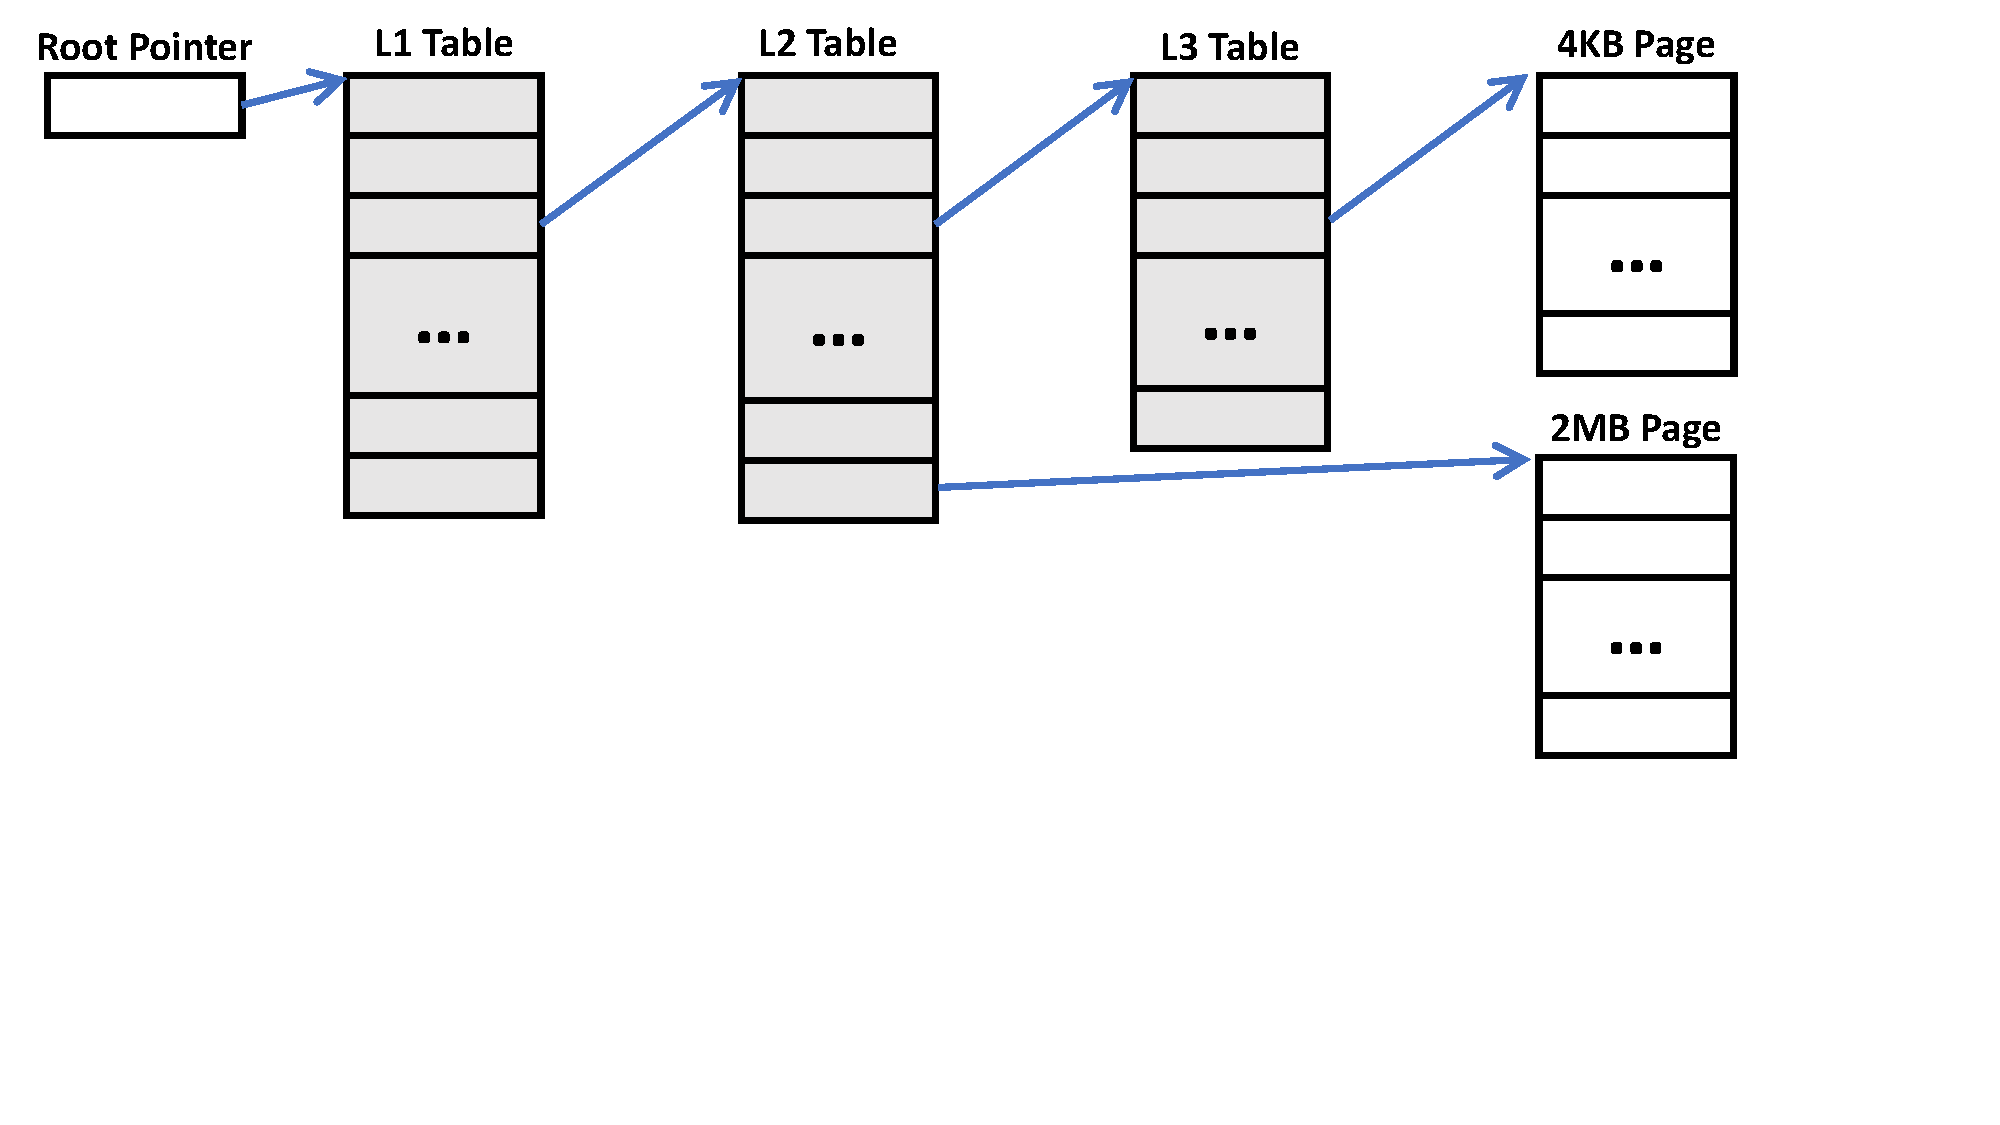
\includegraphics[width=0.8\columnwidth]{fig/hugepage.pdf}
	\caption{Page Table Structure for Variable-sized Pages}\label{fig:hugepage}
\end{figure}

The processor has a data TLB with 64 entries, and each entry can map either a 4KB page or a 2MB page. 
After a TLB miss, a hardware engine walks the page table to reload the TLB. 
The TLB uses a first-in/first-out (FIFO) replacement policy.

You also need to help Li Hua evaluate the memory usage and execution of the following program 
which adds the elements from two 1MB arrays and stores the results in a third 1MB array 
(note that, 1MB = 1,048,576 Bytes):

\begin{lstlisting}
uint8_t A[1048576] = 0; // 1MB array
uint8_t B[1048576] = 0; // 1MB array
uint8_t C[1048576] = 0; // 1MB array
for (int j = 0; j < 1048576; j++) {
	C[j] = A[j] + B[j];
}
\end{lstlisting}

Assume that the A, B, and C arrays are allocated in a contiguous 3MB region of physical memory.
We will consider two possible virtual memory mappings:
\begin{itemize}
	\item 4KB: the arrays are mapped using 768 4KB pages (each array uses 256 pages).
	\item 2MB: the arrays are mapped using two 2MB pages.
\end{itemize}

For the following questions, assume that the above program is the only process in the system, 
and ignore any instruction memory or operating system overheads. 
Assume that the arrays are aligned in memory to minimize the number of page table entries needed. 
The system also is trying to use the least number of page table entries needed.

\begin{parts}

\part[5] \textbf{Virtual Address [5 points]}

This is the breakdown of a virtual address which maps to a 4KB page:\\


\begin{table}[h]
	\centering
	\begin{tabular}{lrlrlrlr}
	42 & 32 & 31 & 21 & 20 & 12 & 11 & 0 \\ \hline
	\multicolumn{2}{|c|}{\quad\quad\quad L1 Index \quad\quad\quad} & \multicolumn{2}{c|}{\quad\quad\quad L2 Index \quad\quad\quad} & \multicolumn{2}{c|}{\quad\quad\quad L3 Index \quad\quad\quad} & \multicolumn{2}{c|}{\quad\quad Page Offset \quad\quad} \\ \hline
	\end{tabular}
\end{table}

Show the corresponding breakdown of a virtual address which maps to a 2MB page. 
Include the field names and bit ranges in your answer.


\begin{table}[H]
	\centering
	\begin{tabular}{lr}
	42 & 0 \\ \hline
	\multicolumn{2}{|c|}{\quad\quad\quad\quad\quad\quad\quad\quad\quad\quad\quad\quad\quad\quad\quad\quad\quad\quad\quad\quad\quad\quad\quad\quad\quad\quad\quad\quad\quad\quad\quad\quad\quad\quad\quad\quad\quad\quad\quad} \\ \hline
	\end{tabular}
\end{table}


\part[5] \textbf{Page Table Overhead [5 points]}

We define page table overhead (PTO) as:

$$
\text{PTO} = \frac{\text{physical memory that is allocated to page tables}}{\text{physical memory that is allocated to data pages}}
$$

For the given program, what is the PTO for each of the two mappings?

$$
\text{PTO}_\text{4KB} = \underline{\quad\quad\quad\quad\quad\quad\quad\quad\quad\quad\quad\quad\quad\quad\quad}
$$


$$
\text{PTO}_\text{2MB} = \underline{\quad\quad\quad\quad\quad\quad\quad\quad\quad\quad\quad\quad\quad\quad\quad}
$$


\part[5] \textbf{Page Fragmentation Overhead [5 points]}


We define page fragmentation overhead (PFO) as:

$$
\text{PFO} = \frac{\text{physical memory that is allocated to data pages but is never accessed}}{\text{physical memory that is allocated to data pages and is accessed}}
$$

For the given program, what is the PTO for each of the two mappings?

$$
\text{PFO}_\text{4KB} = \underline{\quad\quad\quad\quad\quad\quad\quad\quad\quad\quad\quad\quad\quad\quad\quad}
$$


$$
\text{PFO}_\text{2MB} = \underline{\quad\quad\quad\quad\quad\quad\quad\quad\quad\quad\quad\quad\quad\quad\quad}
$$


\newpage
\part[10] \textbf{TLB [10 points]}

Consider the execution of the given program, assuming that the data TLB is initially empty. 
For each of the two mappings, how many TLB misses occur, 
and how many page table memory references are required per miss to reload the TLB?


\begin{table}[h]
	\centering
	\begin{tabular}{|c|c|c|}
	\hline
	Mapping & \quad\quad\quad\quad Data TLB misses \quad\quad\quad\quad & Page table memory references (per miss) \\ \hline
	4KB &  &  \\ \hline
	2MB &  &  \\ \hline
	\end{tabular}
\end{table}



\end{parts}


\pagebreak
\question[20] \textbf{Virtual Memory and TLB [20 points]}


Li Hua creates a machine which is byte-addressed with 20-bit virtual addresses and 16-bit physical addresses. The processor manual only specifies that the machine uses a 3-level page table with the following virtual-address breakdown.


\begin{table}[H]
	\centering
	\begin{tabular}{cccc}
	\quad\quad L1 Index \quad\quad & \quad\quad  L2 Index \quad\quad   & \quad\quad L3 Index  \quad\quad &  \quad\quad Page Offset \quad\quad  \\ \hline
	\multicolumn{1}{|c|}{4 bits} & \multicolumn{1}{c|}{4 bits} & \multicolumn{1}{c|}{4 bits} & \multicolumn{1}{c|}{8 bits} \\ \hline
	\end{tabular}
\end{table}


\begin{parts}
\part[6] \textbf{Physical Address [6 points]}

What is the page size of Li Hua's machine?\\

\underline{\quad\quad\quad\quad\quad\quad\quad\quad\quad}\\


How many bits do physical page number (PPN) and page offset need in physical address, respectively? \\

PPN:\underline{\quad\quad\quad\quad\quad\quad\quad bits \quad\quad}\\   

Page offset:\underline{\quad\quad\quad\quad\quad bits \quad\quad}\\   



\part[14]\textbf{TLB [14 points]}

Li Hua executes the following snippet of code on his new processor. Assume integers are 4-bytes long, and the array elements are mapped to virtual addresses 0x6000 through physical address 0x1FFC. Assume array and sum have been suitably initialized.


\begin{lstlisting}
int List[4096] = 0;
while (1) {
	for (j = 1; j < 5; j++) {
		sum += List[j * 512]
	}
}
\end{lstlisting}


The processor manual states this machine has a TLB with 16 entries. Assume that variables j and sum are stored in registers, and ignore address translation for instruction fetches; only accesses to array require address translation.

In steady state, how many misses from the TLB and total memory accesses will Li Hua observe per iteration of the while loop (lines 3, 4) on average, if (state your reasoning):


\begin{enumerate}
	\item the TLB is direct-mapped \\
	
	Misses from the TLB:\underline{\quad\quad\quad\quad\quad\quad\quad\quad\quad}\\

	Total memory accesses:\underline{\quad\quad\quad\quad\quad\quad\quad\quad\quad}\\

	\quad\\\quad\\\quad\\\quad\\\quad

	\item the TLB is fully-associative (assume LRU replacement policy) \\
	
	Misses from the TLB:\underline{\quad\quad\quad\quad\quad\quad\quad\quad\quad}\\

	Total memory accesses:\underline{\quad\quad\quad\quad\quad\quad\quad\quad\quad}\\

	\quad\\\quad\\\quad\\\quad\\\quad

\end{enumerate}




\end{parts}




\end{questions}
\end{document}
